\documentclass{mscLiterature}
%
%
% Thesis data
%\mscDepartment{Delft Center for Systems and Control (\textsmaller{DCSC})}%
\mscProgram{Systems and Control}
%Change if needed to
%\mscProgram{Mechanical Engineering}
\mscFaculty{Mechanical, Maritime and Materials Engineering (3mE)}%
\mscName{Yudha Prawira Pane}%
\mscDate{\today}%
\mscTitle{Reinforcement Learning for Tracking Control in Robotics}%
%\mscSubTitle{Optional Subtitle}%
\mscKeyWords{reinforcement learning, tracking, optimal control, constraint}% only used in PDF properties
\mscCoverPicture{STYLESTUFF/COVER}% to place a picture ( here the example COVER.eps) on the back of the cover page
%
%
% Third party options (create text/logo on the copywrite page)
\mscThirdPartyText{The implementation work in this thesis was done at DCSC's robotics lab.}
\mscThirdPartyLogo{STYLESTUFF/EXAMPLELOGO}
% NOTE: on the title page only the TU Delft logo is permitted.
%
%
%
% Finalize the thesis data
\setThesisInfo
%
% Use \includeonly{} to build only certain parts of your thesis
%\includeonly{introduction, real_chapter, empty_chapter, long_chapter}%
%
%PH Toegevoegd 24-10-2011
%allow (matlab) listing max 1pt flexibility between lines
\lstset{lineskip=0pt plus 1pt minus 0pt}
%
\usepackage[]{algorithm2e}
\usepackage{graphicx}
\usepackage{caption}
\usepackage{subcaption}

\begin{document}
%
%========================== Front matter ======================================
\frontmatter %
%
% Make the cover page and hell of a lot of title pages
\maketitle
%
%
% Abstract (does not appear in the Table of Contents)
\chapter*{Abstract}%

Reference or trajectory tracking is one of the requirements in order to carry out a complex robotic task. Capability to perform a precise tracking with minimum possible error is crucial for the robots that are to be deployed at manufacturing industries such as semiconductor, automotive and recently, an emerging application of 3D printing.

The approach used in the past has been to design model based controllers which involve feedback and feedforward control or more recently, a predictive control. The drawback of such scheme, however, lies on the requirements of system model as a slight model mismatch could lead to poor tracking performance. For a repetitive control error, researchers have designed the so called Iterative Learning Control (ILC). In this literature study, a new method to optimize the tracking performance of nominal controller using reinforcement learning (RL) is proposed. 

Throughout the literature study, the existing work for RL-based tracking control clusters into 3 approaches: RL for optimal tracking (Lewis et al.), RL-based dynamic tuning (Brujeni et al.), and nonlinear compensator via RL (Bayiz et al.). The advantages, limitations and practical challenges of the 3 approaches are discussed. These criterion serves as a basis to select one method which will be developed and implemented during the thesis. Furthermore, the testbed for the thesis which is a UR5 3D printing robot is also presented. Finally, the literature study concludes with the research plan and discussion.
%
% table of contents, (\toc of \toclof of \tocloflot )
\tocloflot
%
%
%
% Preface
\chapter{Preface}
This thesis came into existence after a long wander to search for a topic which suits my vision. I have always wanted to start my own robotics company some day. So the first thing that I decided was that my master thesis should have a strong practical work. To meet this goal, I set up an appointment with Subbu in his office where he explained to me about the topics which were available at the \ac {DCSC} robotics lab. At first, my topic was going to be "\ac {RL} for underactuated robot". Sounds novel and interesting. However, in terms of feasibility, this topic might become hard since there is only one underactuated robot in the lab, the slacklining robot, and it was not in a ready-to-program state. This means that I would have to spend much time making sure the robot work before I can apply my controller. Prof. Babu\v{s}ka then offers me a slightly similar topic but with totally different test bed. This is when I came into \ac {RL} for tracking control. This is a quite new topic in control field since only few people have conducted researches on it. After an hour of discussion, it is decided that this will be my thesis topic. The topic offers both theoretical and practical aspects since I will get a chance to apply my solution to a real robotic setup, UR5 from Universal Robots. Now that I am finishing my literature survey, I hope that I would deliver a satisfying result at the end of the thesis.

\vspace{30mm}
Delft, University of Technology \hfill \mscname \\
\mscdate
%
% Acknowledgements
\chapter{Acknowledgements}%

I would like to thank my supervisor Prof. Dr. Ir. R. Babu\v{s}ka for his guidance in defining my thesis topic and his valuable advices during the literature study.

I would also like to thank Subramanya Nageshrao (Subbu) for being a patient and resourceful daily supervisor. His advices help me a lot while encountering problems.

\vspace{30mm}
Delft, University of Technology \hfill \mscname \\
\mscdate
%
% Dedication page. 
\cleardoublepage
\thispagestyle{empty}
\vspace*{\stretch{1}}

% Put your own motto here, or dedicate your work to your Mom or whatever...
\begin{quote}
\noindent``In the future, airplanes will be flown by a dog and a pilot. And the dog's job will be to make sure that if the pilot tries to touch any of the buttons, the dog bites him.''
	
--- \emph{Scott Adams}
\end{quote}

\vspace{\stretch{3}}
\clearemptydoublepage
%
%========================== Main matter ======================================
\mainmatter
%
%
% Introduction
\chapter{Introduction} \label{chap::intro}
Reference or trajectory tracking is one of the building blocks to perform a complex task in robotics. Given a desired path/trajectory, the robot must be able to follow it as quickly as possible with minimum error. Capability to perform this precise tracking is crucial for robots that are to be deployed at manufacturing industries such as semiconductor, automotive, and recently, the emerging application of 3D printing. 

Statistics by International Federation of Robotics (IFR) \cite{IFR2014} shows that the global sales of industrial robots continues to increase steadily. In 2014, it is expected that the total number of industrial robots installed reaches 205,000 units, a rise of approximately 15 \% from previous year. The survey points out that the mature markets such as automotive, electronics, and metal are responsible for such growth. 

Meanwhile, there is also a growing interests in applying robots to relatively new applications such as 3D printing, architecture, and art. For instance, research done by Gramazio et. al \cite{Helm2014} \cite{Lloret2014} aims to push the capability of industrial robots to make direct fabrication based on CAD model a reality. The advantage of using robots over conventional CNC machines lies on their flexibility, easy-to-adapt feature, and high \ac{DoF} -- enabling execution of difficult configuration in \ac{3D} space. These aforementioned applications demand high precision since a minuscule of error could lead to a defect product or even worse, a disaster. Therefore a precise, accurate reference tracking capability is inevitable.

In order to achieve this, a reference tracking control is needed. However, a robot brings along non-linearities, noises, and external disturbances that are difficult to model, let alone compensate. This unknown properties often hinders the controller to perform optimally. A class of controllers which solely depends on the system's model will surely suffer a poor tracking accuracy. The natural answer to this problem is to introduce a controller capable of adjusting its parameter overtime by comparing the reference to the actual trajectory. By doing so, the controller will have an extra degree of freedom to compensate for the unknown properties hence improving the tracking quality. The controller of such characteristic belongs to the class of adaptive controller.

In this thesis, a method to improve the performance of nominal controller by using \ac{RL} is proposed. Despite decades of extensive research on \ac{RL}, its application to optimize tracking problem in robotics is still a relatively unexplored topic. Based on the literature, there are three potential approaches to address the tracking problem. The first one comes from the work of Lewis et. al. on \ac{RL} for optimal control. Lewis and his group have been developing a comprehensive research on \ac{RL} for solving the solution to adaptive optimal control. Their research has been extended for discrete \cite{Kiumarsi20141167} and continuous time \cite{Modares6760477}, for linear \cite{Kiumarsi6760476} and non-linear system \cite{Kiumarsi6918527}. Furthermore, their technique could also be applied in Q-learning \cite{Kiumarsi20141167} and actor-critic structure \cite{Kiumarsi6918527}. The second approach is proposed by Bayiz et. al. in \cite{Efe2014}. The paper discusses a slightly different approach by using \ac{RL} to learn disturbance compensation for nonlinear system. This disturbance compensation acts as an additive input signal to the control signal. Finally, the third approach uses the notion of adaptive gain scheduling. Buchli et.al present an algorithm called \ac{PI$^2$} to vary the gain of a \ac{PD} controller in order to achieve a desired terminal state \cite{Buchli2010} \cite{Buchli6037312}. Having explained the motivation of this thesis, now we are ready to define the research problem.



\section{Problem Definition}
The fundamental problem in this literature study concerns the non-optimal performance of nominal controller with respect to reference tracking task. Hence the research question can be raised as follows.

\textit{"Is it possible to integrate Reinforcement Learning technique to a nominal controller in a certain structure such that reference tracking performance of the controlled system significantly improves?"}

While conducting a research, it is often wise to restrict oneself to a simple context, but still captures the essential elements of the original problem \cite{einstein}. Therefore, in answering this question, some simplifying assumptions are made.

\begin{enumerate}
	\item The system to be controlled is fully actuated
	\item The system to be controlled is observable. This assumption is necessary in order to satisfy Markov property \cite{sutton1998reinforcement}.
	\item Nominal, stabilizing controller is available	
	\item Identification reveals some information about the system, but alone is not adequate to design an accurate reference tracking controller.
\end{enumerate}

\section{Goal of the Thesis}

The goal of this thesis are as follows:
\begin{enumerate}
\item To provide a general framework of improving tracking control using \ac{RL}
\item To apply and compare existing method of \ac{RL} for tracking application to the 3D printing robot setup
\item To come up with modification or improvement of previous methods
\end{enumerate}

\section{Literature Study Approach}
In order to build a strong theoretical foundation for later implementation, the following literature approach is used. The order does not necessarily represent a sequential process.
\begin{enumerate}
	\item To gather as many relevant papers as possible from reputable academic search engines. Relevant means papers which deal with \ac{RL} and control system. Additional pointer to tracking problem is heavily considered. Examples of sources being used are Web of Science, IEEE Xplore and Google Scholar.
	\item To discuss the detail of future experimental setup (UR5 \ac{3D} printing robot) with Marco de Gier, who was working on the setup at the time this literature is written.
	\item From the papers, extract existing methods which have the potential for application to the future experiments. So far, there are 3 different methods that are considered. These methods will be explained in detail in Chapter \ref{chap::survey}.
	\item Create simple simulation programs showing how each method works
	
\end{enumerate}


\section{Outline}

The structure of this literature review is arranged as follows. In the next chapter, an introductory materials of \ac{RL} is presented. This covers the framework widely used in \ac{RL} (Markov Decision Process), the principle of value and policy iteration, the formulation of \ac{RL} for continuous space, and the actor-critic structure which suits the framework of control system. Chapter \ref{chap::survey} provides the result of literature study being conducted. This includes the detailed explanation of methods found and their comparison. Furthermore, a new controller is proposed. 

%\section{Nomenclature}



\chapter{Reinforcement Learning Preliminaries}
This chapter is dedicated to present a concise theory of reinforcement learning. The first section will show how a certain goal can be formalized as a reward maximization -- one of the ideas which serves as a basic foundation of \ac{RL}. Section \ref{sec:mdp} explains the basics of \ac{MDP}, a general framework used in \ac{RL} problem. Subsequently, an intuition of value and policy iteration will be developed in section \ref{sec:value_iter}. The fourth section will present the extension of \ac{RL} for continuous space. Finally, section \ref{sec:actor} will discuss the actor-critic structure which is a natural representation for control system problem.

\section{The Principle of Maximizing Cumulative Reward}
The nature of \ac{RL} is inspired by the way living organisms learn to reach their desired goals by first acting on the environment, observe the changes that occur, and reward their action accordingly. if tThe idea of \ac{RL} is to 

\section{Markov Decision Process} \label{sec:mdp}
\ac{MDP} is defined as a tuple which satisfies Markov property. The detailed explanation of this property can be found on \cite{sutton1998reinforcement} section 3.5 but the main idea is that to determine the probability of a state at certain time, it is sufficient to know only the state of previous time instant. This probability is mathematically denoted in Equation \eqref{eq:markov}.

\begin{equation}
	\text{Pr}\{x_{t+1} = x', r_{t+1} = r| x_t, u_t \}
	\label{eq:markov}
\end{equation}
where $x$ denotes state, $u$ denotes action, and $r$ denotes immediate reward obtained upon applying the input on the corresponding state.

\section{Value and Policy Iteration} \label{sec:value_iter}

\section{Reinforcement Learning for Continuous Space}
\subsection{Function Approximation}


\section{Actor-Critic Structure} \label{sec:actor}

%
% A Real Chapter
\chapter{Reinforcement Learning for Tracking Problem: A Survey}

This is real chapter for \ac{DCSC}, ok? We will use it as a demo for the different headings you can use to structure your text.


\section{Dynamic Tuning via Reinforcement Learning}
This is the first section .

\subsection{Case Study: PI Tuning using Reinforcement Learning}
This is the subsection of the first section.

\section{Nonlinear Compensation for Tracking via Reinforcement Learning}
This is second section.
\subsection{Case Study: 1-DOF Robot Gravity Compensation}

\section{Reinforcement Learning for Optimal Tracking Control}
This is third section.

\section{Self-Proposed Controller [tentative]}


\chapter{Experimental Setup} \label{chap:testbed}

The purpose of this chapter is to present the 3D printing robot system used as the testbed. The robotic system consists of a UR5 robot manipulator, 3D print head, and a laser scanner -- each will be described in Section~\ref{sec:ur5}. In Section~\ref{sec:current_work}, we will discuss the previous works done on the robotic system. This includes the system identification model and the \ac {MPC} controller. Finally, based on the we will formalize the hypothesis in Section~\ref{sec:hypo}.
\section{The 3D Printing Robot System} \label{sec:ur5}
\subsection{UR5 Robot Arm}
UR5 is a lightweight, flexible industrial robot from Universal Robots. The robot is chosen due to its human-safe operation with a quite good repeatability of 0.1 mm \cite{UR5}. The robot is a serial link 6 \ac{DoF} manipulator with internal controller to take care of the gravity compensation and most of the non-linearities. In general, the robot can be controlled like a system of 6 decoupled servos, although this is only correct to some degree. We will explain later why this is the case.

Since the internal controller can not be "seen", let alone modified, the UR5 and the controller are viewed as one system. The \ac {RL} controller will be implemented in MATLAB which communicates with the UR5 using a TCP/IP protocol on 125 Hz frequency. There is a number of ways to send control command to the robot:
\begin{enumerate}
\item Tool position commmand \\
The tool position means the position of the robot's end effector in Cartesian coordinate. The origin of the Cartesian frame is exactly at the robot's base. Figure~\ref{fig:UR5_Robot01} shows a full posture of the UR5 robot. With this type of control input, one can command the end effector to move to a specified tool position $ s = (x, y, z) $ in mm. This type of command results in a smooth motion if applied in a long sampling period (> 1 second). For the 125 Hz communication rate, however, it suffers from a poor jitter.

\item Tool speed command \\
The tool speed command is in the same coordinate as the position command, but now the control input is the velocity of the end effector in mm/s. This command results in a much smoother motion compared to position command.

\item Joint position command \\
This command controls the joint position of individual robot's joint to a specified angle in radian. Similar to tool position command, it results in a jerky motion. 

\item Joint speed command \\
This command drives the individual joint into the desired joint velocity in the unit of radian/s. This results in the smoothest motion compared to others. Due to this reason, this command will be used to drive the robot throughout the thesis.

\begin{figure}
\centering
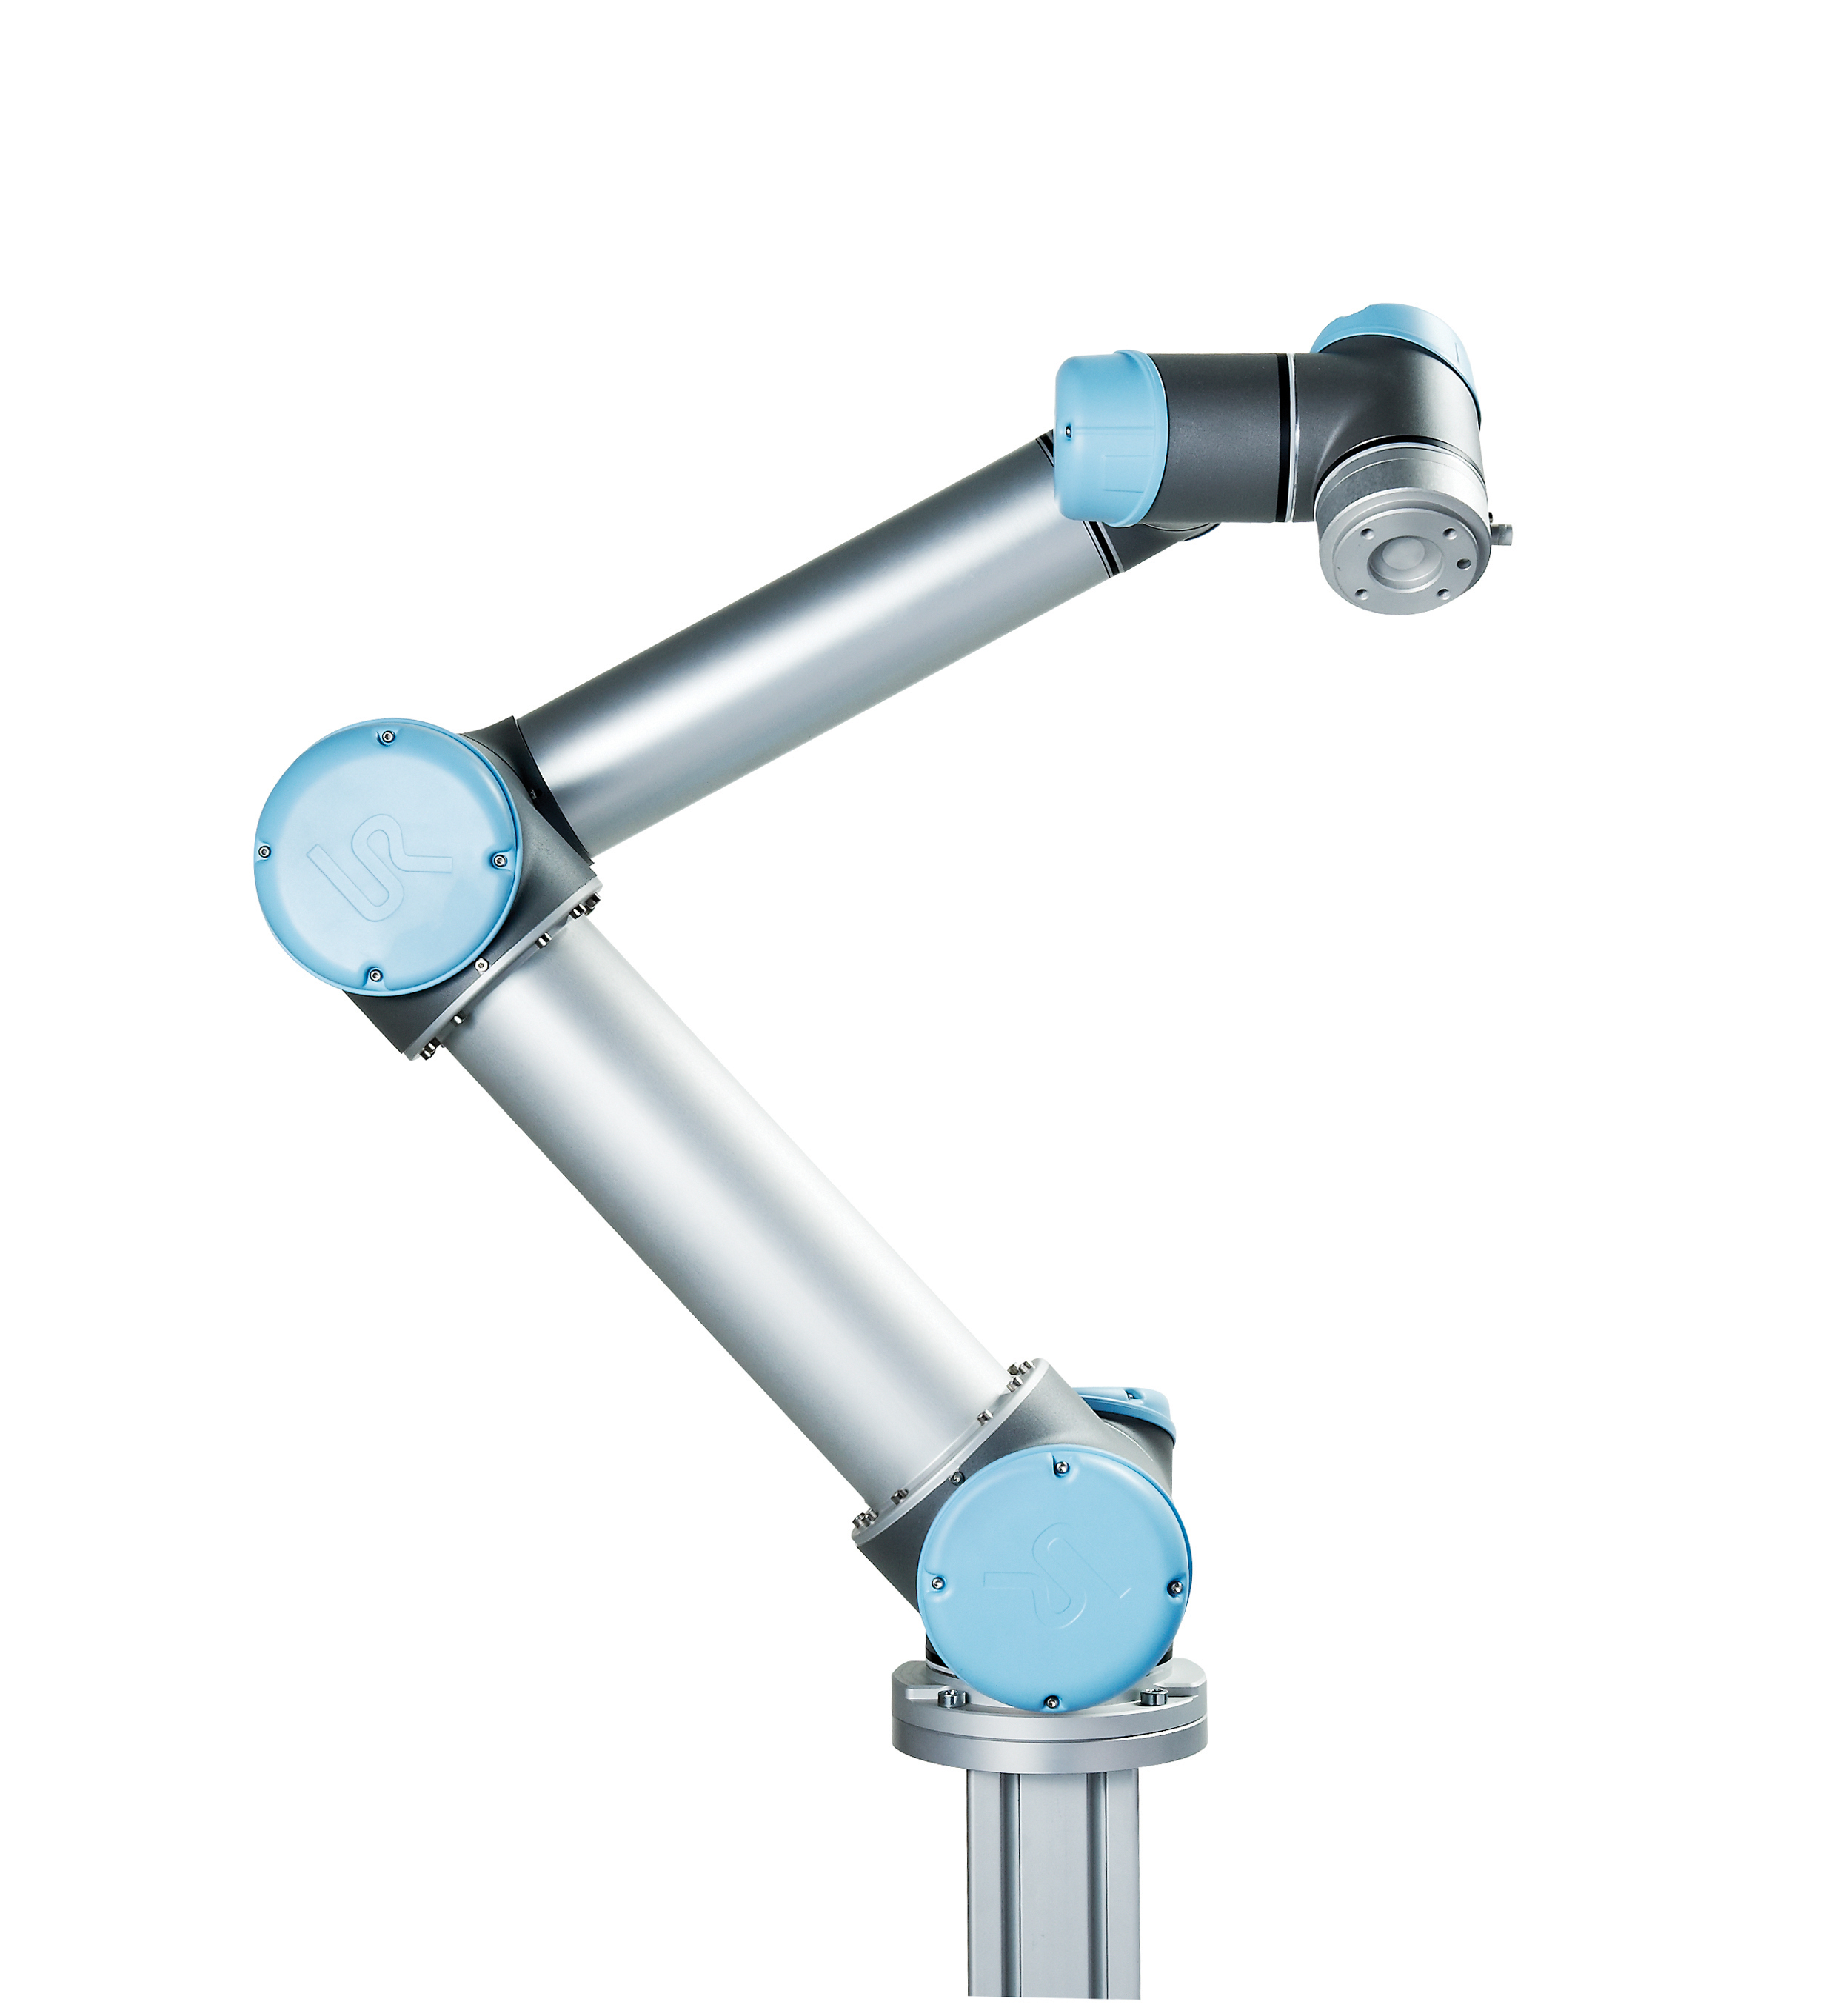
\includegraphics[width=0.5\linewidth]{UR5_Robot01}
\caption{The UR5 Robot (photo courtesy of Universal Robots)}
\label{fig:UR5_Robot01}
\end{figure}
 
\end{enumerate}

\subsection{Laser Scanner}
The laser scanner is a scanCONTROL 2700-25 series laser manufactured by Micro-Epsilon and mounted on the robot's end effector. It offers a 100 Hz profile frequency, up to 64,000 measuring points per second and 4 $ \mu $m scanning resolution. The laser scanner is used to generate the 3D point cloud of the surface we would like to print on and to measure the tracking accuracy. Figure~\ref{fig:scanCONTROL} shows the 3D view of the laser scanner.

\begin{figure}
	\centering
	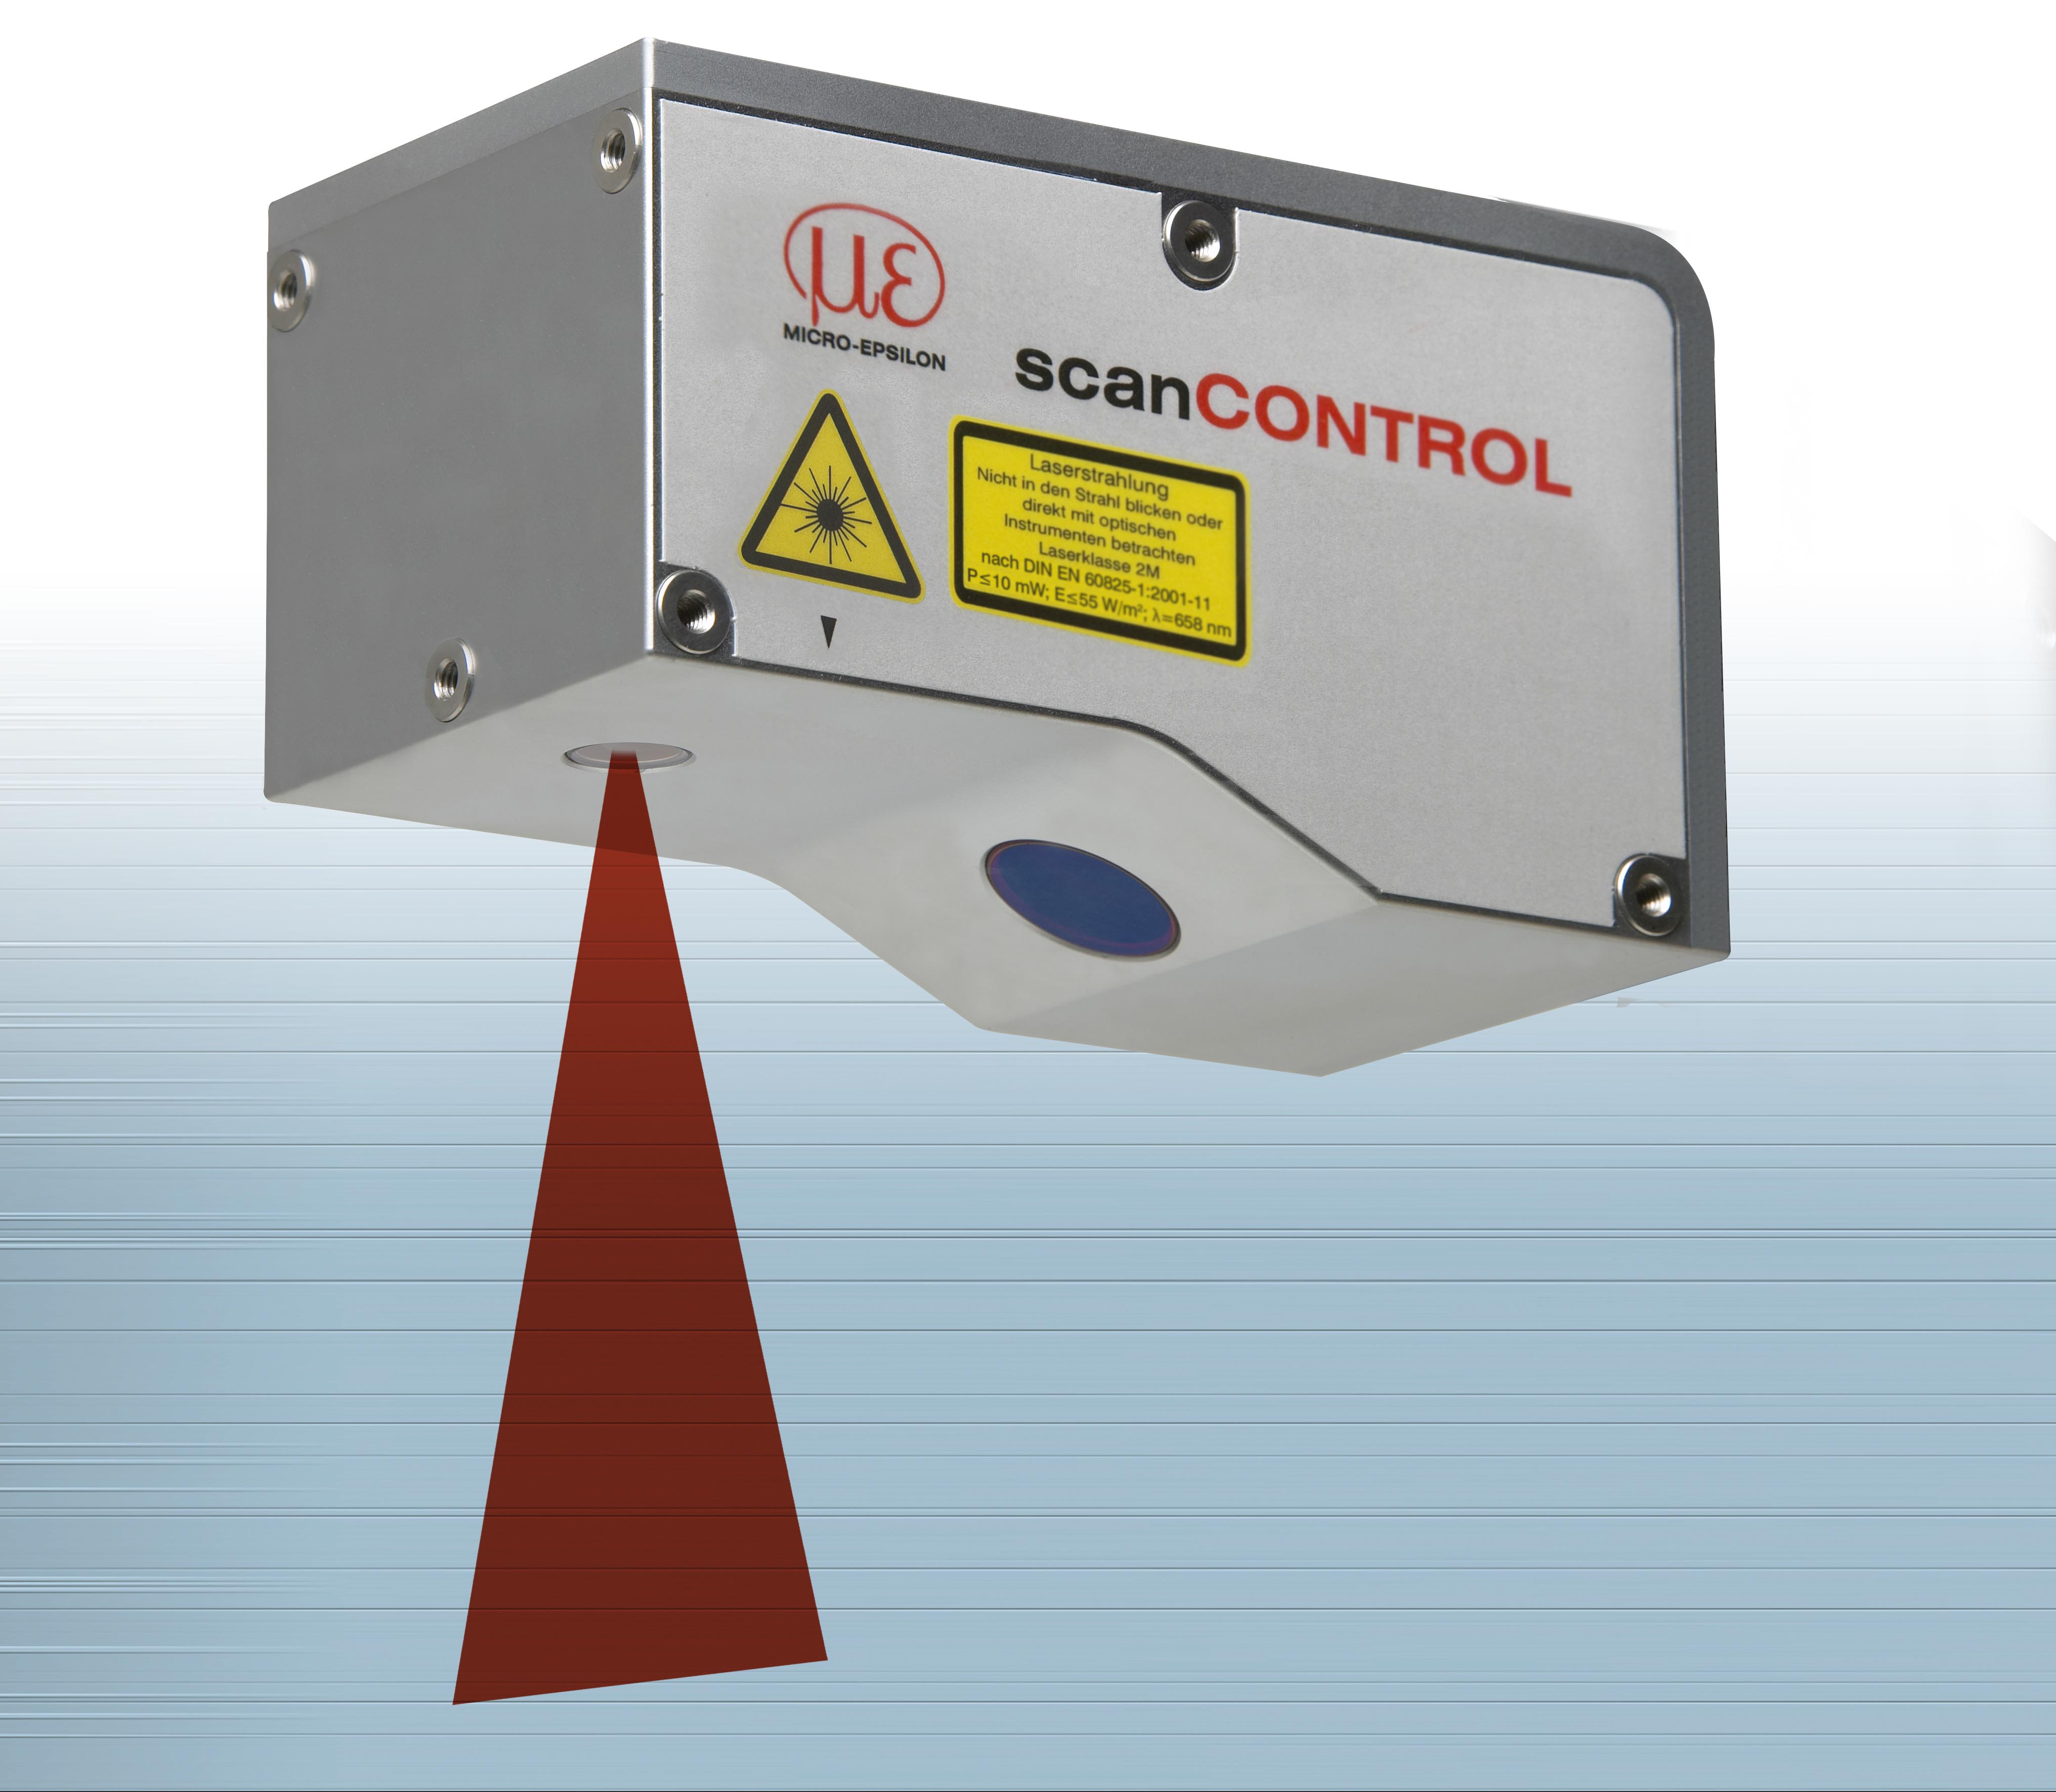
\includegraphics[width=0.5\linewidth]{scanCONTROL}
	\caption{scanCONTROL 2700 series laser scanner (photo courtesy of Micro-Epsilon)}
	\label{fig:scanCONTROL}
\end{figure}

\subsection{3D Print head}
The 3D print head is a Cobalt C29 inkjet printhead developed by Oc{\'e} Technologies B.V.  Since the print head does not contribute to the controller design and implementation, it will not be used throughout the thesis. Figure~\ref{fig:ur5-endeffector} shows the robot's end effector with print head attached \cite{sunniva2013}.


\begin{figure}
\centering
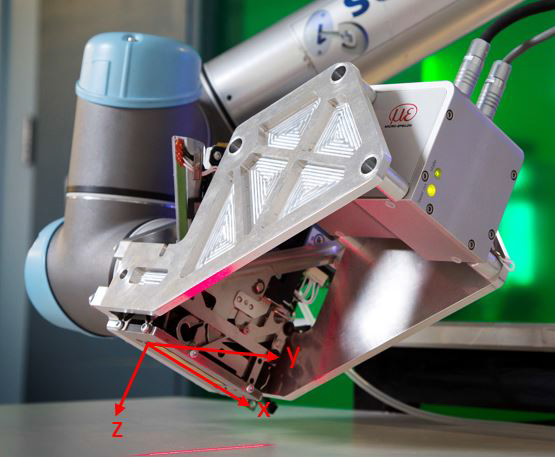
\includegraphics[width=0.5\linewidth]{ur5}
\caption{The end effector of the UR5 robot with 3D print head and laser scanner attached (photo courtesy of Sunniva Ipenburg)}
\label{fig:ur5-endeffector}
\end{figure}

\section{Previous Work} \label{sec:current_work}
In this section, we will present a short overview of the previous works done by de Gier from \ac {DCSC}, specifically on the system identification and the \ac {MPC} controller \cite{Gier2013}.

\subsection{System Identification}
An important assumption for the identification is that the robot acts as six decoupled servos along with their internal controller. Additionally, it is also assumed that each joint is a \ac{LTI} system. This implies that there will be six individuals \ac {LTI} model to identify. Each model is a \ac{SIMO} system with the joint velocity reference $\dot{\theta}_r$ as the input and joint position $\theta$ and velocity $\dot{\theta}$ as the outputs. 

For this purpose, a subspace identification method is used. According to the significant singular values, the order of each model is determined to be either 4 or 5 \cite{verhaegen2007filtering}. After the models are obtained, each joint model is then validated using a square input signal while the other joint angles are held constant. The \ac{VAF} values of each joint for the validation test is shown in Table~\ref{tab:vaf}. Although the result shows a quite good \ac {VAF} score, it is still not good enough to achieve a perfect tracking. To give an example of the performance, the model validation plot of joint 1 and 5 is shown in Figure~\ref{fig:idenJoint}.

\begin{table}[h!]
\caption{\ac {VAF} scores of the simulated outputs for all joints}	
	\centering
	\begin{tabular}{|c|c|c|}
		\hline Joint & Position  & Velocity \\ 
		\hline 1 & 98.64 & 87.33 \\ 
		\hline 2 & 98.05 & 88.33 \\ 
		\hline 3 & 98.55 & 88.47 \\ 
		\hline 4 & 98.97 & 89.50 \\ 
		\hline 5 & 99.46 & 90.32 \\ 
		\hline 6 & 98.87 & 85.13 \\ 
		\hline 
	\end{tabular} 
	\label{tab:vaf}
\end{table}


\begin{figure}
	\centering
	\begin{subfigure}[b]{0.4\textwidth}
		\includegraphics[width=1\linewidth]{"../../Progress Report/Joint5"}
		\caption{}
		\label{fig:Joint5}
	\end{subfigure}%
	~ %add desired spacing between images, e. g. ~, \quad, \qquad, \hfill etc.
	%(or a blank line to force the subfigure onto a new line)
	\begin{subfigure}[b]{0.4\textwidth}
		\includegraphics[width=1\linewidth]{"../../Progress Report/Joint1"}
		\caption{}
		\label{fig:Joint1}
	\end{subfigure}
	\caption{Model validation of joint 1 and 5 for joint position and velocity}\label{fig:idenJoint}
\end{figure}

\subsection{\ac{MPC} Controller}
The previous work involves a design and implementation of \ac {MPC} controller. \ac {MPC} proves to perform better than e.g. \ac{PID} but tracking error is still present in the form of jitter.


\chapter{Research Direction and Discussion}

This chapter presents the result of the literature study. It starts in Section~\ref*{sec:review} by presenting the review and analysis of the three \ac {RL} approaches explained in Chapter~\ref{chap::survey}. The review consists of parameters that are taken into considerations -- advantages, limitations and practical challenges for implementation. Section~\ref{sec:res_planning} presents the research plan which will be carried out during the thesis. In the end of the chapter, a discussion is covered in Section~\ref{sec:discussion}
\section{Review and Analysis of \ac{RL} Approaches} \label{sec:review}
\subsection{{\ac{RL} for Optimal Tracking Control}}
From the mathematical perspective, the optimal tracking approach is more rigorous compared to the other two. The proof of convergence, for instance, has been provided in literature \cite{1099755}. Another advantage is since the approach is based on lyapunov function, system's stability is guaranteed. Furthermore, researchers have successfully extended this approach to different control condition: discrete-continuous time, linear-nonlinear system, known-(partially)unknown model. From all of these benefits, the optimal tracking approach seems to be a suitable choice. However, there are some limitations which must be overcome in order to implement this method for a robotic tracking application.

As previously stated in the motivation, the goal of the thesis is to push the envelope of current tracking performance using \ac {RL}. As for the case-specific, it is hypothesized in Chapter~\ref{chap:testbed} that the low tracking performance is due to unknown non-linearities and disturbance in the robot. Therefore, a model-based standard optimal tracking is no longer a relevant solution. Although \cite{Kiumarsi20141167} has shown that using \ac{RL}, one can obviate the need of system model for linear system, the solution for an unknown non-linear system is not yet available. This is one crucial limitation to this method for now since we actually want to improve tracking of potentially non-linear system. Even if the solution exists, a practical problem will most probably arise due to the necessity of persistence of excitation in order to achieve a converging control policy \cite{Kiumarsi20141167} \cite{AlTamimi2007473}. For the UR5 robot testbed, this could potentially damage the robot since the motors must be excited with a persistently exciting signal such as pseudo-random noise. 

The second limitation of the approach is that it is still not known how to integrate the available but inaccurate model to the optimal tracking. Literatures have shown that although the models are not perfect, it can still help in speeding up the \ac {RL} convergence time \cite{Brujeni5669655} \cite{Grondman6096441}. Therefore, model integration would be a useful, though not necessary factor. Due to these factors, optimal tracking \ac {RL} is not the most suitable method for the thesis requirements.

\subsection{Dynamic Tuning via \ac{RL}}
\subsubsection{Direct Tuning of Nominal Controller}
The advantage of the direct tuning by \ac{RL} is its simple, intuitive scheme and rather direct implementation. However, direct tuning \ac{RL} only works with a standard state/output feedback controller such as \ac{PID}. State/output feedback controller is known for its nature which is always "late" since it has to wait for the error to appear and then compensate for it. Throughout the literature survey, author could not find a paper which integrates an \ac{RL}-based dynamic tuning with more sophisticated controller such as optimal tracking control or \ac {MPC}. Due to this bottleneck in performance, the direct-tuning is not the best choice to answer the research's goal.
\subsubsection{Gain scheduling for \ac{DMP}}
As previously explained in Chapter~\ref{chap::survey}, \ac{PI$^2$} learns the optimum trajectory to enable robotic manipulator passing through a certain intermediate point described by \ac{DMP}. In order to use \ac{PI$^2$} \ac{DMP} for reference tracking, one would need to extend the point of attractor $g$ into a full trajectory $g(k)$. The answer of this problem, assuming that the question itself is relevant, is not present at this time.

In order to provide an answer to above problem, a thorough understanding of the \ac{PI$^2$} algorithm and \ac {DMP} approach is needed. This is a particularly challenging problem since to derive the \ac{PI$^2$} itself involves a rather complex procedures such as stochastic optimal control which can easily be misunderstood if not treated carefully \cite{Buchli2010}. Due to the needs of extensive theoretical study, duration constraint of the thesis and the risk that this method is ultimately irrelevant, it is decided that \ac {PI$^2$} \ac{DMP} is not the most suitable solution.

\subsection{Nonlinear Input Compensation via \ac{RL}}
To the best of author's knowledge, there is no any literature yet which addresses the implementation of this method to a full reference tracking task. The only existing work is presented in \cite{Efe2014} which compensates an unknown gravity for a \ac {PD}-controlled 1-\ac {DoF} robot arm acting on a simple step command. Thus, this method, if successfully implemented, can be considered a novel solution. This algorithm is also modular in the sense that the compensator acts as an additive signal which does not influence the controller's output. This means the better the nominal controller performs, the smaller tracking errors needs to be compensated. Furthermore, the compensator also does not require any information about the system model to operate. 

The drawback of this method is the lack of mathematical formalization to prove the common control criterion: stability, convergence and robustness. From the practical point of view, some kind of mechanism must be introduced to ensure that the compensator signal is not too large since the nominal controller has already performed near optimally. Nevertheless, due to the model-free characteristic, this method is chosen to be the solution which will be developed and implemented for the rest of the thesis.

\section{Research Plan} \label{sec:res_planning}
The post-literature survey research plan is organized as follows. Before commissioning the implementation on the UR5, a simple simulation of a 1-\ac {DoF} manipulator will be programmed. The purpose of the simulation is to verify that the proposed method is actually working. If the \ac{RL}-based optimizer indeed works, the next step would be to further develop the controller for implementation on the UR5 robot. If the controller performs as expected, improvement will be carried out until the end of the thesis. Parallel to these steps, the thesis report will be written as well. The research plan is summarized in a flowchart as shown in Figure~\ref{fig:flowchart}.

\begin{figure}
\centering
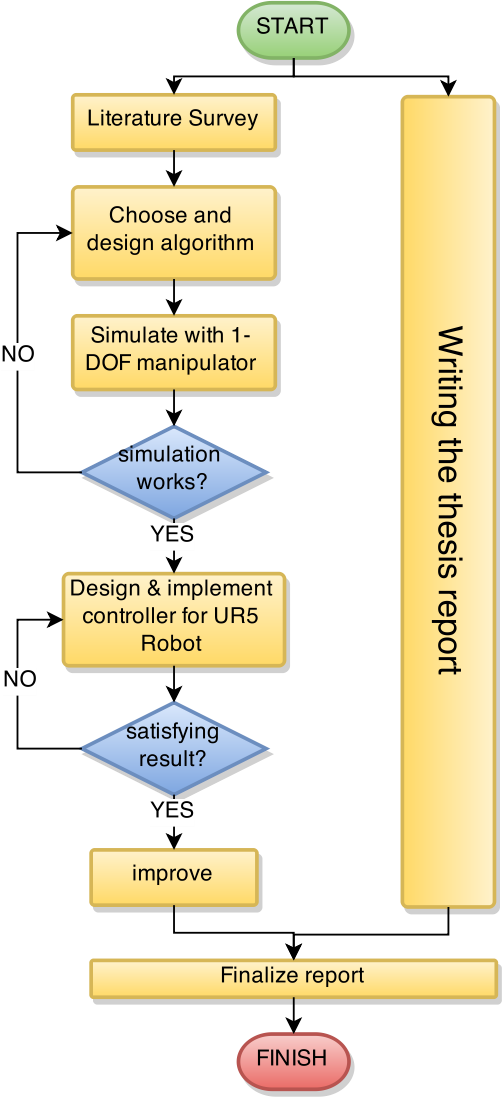
\includegraphics[width=0.5\linewidth]{Drawing1}
\caption{Research plan flowchart}
\label{fig:flowchart}
\end{figure}

\section{Discussion}\label{sec:discussion}
Since Chapter~\ref{chap:testbed} has shown that for a simple straight line trajectory the jitter appears to be repetitive, author finds it interesting to compare \ac{RL} for reference tracking with a much more mature technique, namely \ac{ILC} \cite{4048052}. As the name suggested, \ac {ILC} is developed to improve tracking contaminated by repetitive error/disturbance. This method has been successfully implemented for various applications from CNC machining \cite{299157} to industrial robots \cite{1044377}. Therefore, \ac {ILC} could serve as a benchmark during later verification.

\chapter{Future Work and Experiments Plan}

%\section{Experimental Setup: UR5 Robot}



\chapter{Conclusion}
Despite having used for various applications for decades, the application of \acs {RL} in control still has much space to explore. In this thesis, a subset of that space, namely reference tracking problem is addressed. The search for existing works results in 3 methods which must be analyzed carefully in order to obtain a strong motivation to finally choose one of them. The \acs {RL}-based optimal tracking is mathematically more convincing than the other two. Not only that it will surely converge, a stability can also be guaranteeed. In the other hand, the dynamic tuning methods have problems with performance and feasibility. The direct tuning is intuitive and relatively easy to implement, but it will perform less since it depends on a feedback controller which will always be late in compensating error. The \acs{PI$^2$} method has successful track-record for variable impedance control task, but rather unconvincing for tracking problem. Finally, the additive tracking problem is chosen since it strongest represents the nature of \acs {RL} which does not depend on the system model. This method enables an additional degree of freedom to optimize the controller, independent from the nominal controller itself. Furthermore, it is considered interesting to compare the \acs{RL}-based tracking controller with a more widely known \acs{ILC}.
%
%
%========================== Appendices =======================================
\appendix
%
\chapter{Appendix}

Appendices are found in the back. 

\section{Simulation Program}

\subsection{A MATLAB listing}

\lstset{language=matlab}
\lstinputlisting{test.m}


%========================== Back matter ======================================
\backmatter
%
% Bibliography
\bibliographystyle{ieeetr}
\bibliography{MyBib}

%
%
% Glossary
\chapter{Glossary} %
%
\printacronyms
\begin{acronym}[\hspace{0.8in}] % 0.8in is also used by the nomenclature
	\acro{3D}{3-dimension}	
	\acro{3mE}[3\textlarger{m}E]{Mechanical, Maritime and Materials Engineering}%
	\acro{AMS}{American Mathematical Society}%
	\acro{ARE}{algebraic Riccati equation}	
	\acro{DCSC}{Delft Center for Systems and Control}%	
	\acro{DMP}{dynamic movement primitive}
	\acro{DoF}{degrees of freedom}%
	\acro{DP}{Dynamic Programming}
	\acro{HJB}{Hamilton-Jacobi-Bellman}
	\acro{ILC}{iterative learning control}
	\acro{ISE}{integral of squared errors }
	\acro{LLR}{local linear regression}
	\acro{LQT}{linear quadratic tracking}
	\acro{LTI}{linear time-invariant}	
	\acro{MDP}{markov decision process}%
	\acro{MIMO}{multi-input multi-output}
	\acro{MLAC}{model learning actor-critic}
	\acro{MPC}{model predictive control}
	\acro{PD}{proportional derivative}		
	\acro{PDE}{partial differential equation}
	\acro{PI}{policy iteration}	
	\acro{PI$^2$}{policy improvement with path integral}
	\acro{PID}{proportional-integral-derivative}
	\acro{RL}{reinforcement learning}%
	\acro{SAM}{stochastic action modifier}
	\acro{SARSA}{state-action-reward-state-action}
	\acro{SIMO}{single-input multi-output}
	\acro{SISO}{single-input single-output}	
	\acro{TD}{temporal-difference}	
	\acro{TU}[TU D\textlarger{elft}]{Delft University of Technology}%
	\acro{VAF}{variance accounted for}
	\acro{VI}{value iteration}
\end{acronym}%
%
%
% Nomenclature
\printnomencl%
%
% Index
\cleardoublepage
\printindex

\end{document}
